\documentclass[xcolor=dvipsnames]{beamer} 



%\usepackage{beamerthemesplit}
\mode<presentation>
{
  \usetheme{Antibes}
  \usecolortheme[named=OliveGreen]{structure} 
  % or ...

  \setbeamercovered{transparent}
  % or whatever (possibly just delete it)
}

\usepackage[polish,english]{babel}
\usepackage[utf8]{inputenc}

% greetings, introduce yourself

\title[WR Project Status\hspace{2em}\insertframenumber/
\inserttotalframenumber]{The White Rabbit Project}

\subtitle{Technical introduction and status report}
\author{T. Włostowski}
\date{November 11, 2010}

\institute%[Universities of Somewhere and Elsewhere] % (optional, but mostly needed)
{
  BE-CO Hardware and Timing section\\
  CERN
 }

\pgfdeclareimage[height=0.5cm]{wr-logo}{wr-logo.jpg}
\logo{\pgfuseimage{wr-logo}}
\AtBeginSection[]
{
  \begin{frame}<beamer>{Outline}
    \tableofcontents[currentsection]
  \end{frame}
}

\begin{document}

\frame{\titlepage}

% wr is a multilab, multicompany project which aim is to build next-gen control&timing network based on ethernet.

\section{Introduction}
% Layer 2 and it's for free - transparent. Data, sycchronism, determinism
\begin{frame}{Origin of the name}
\begin{center}
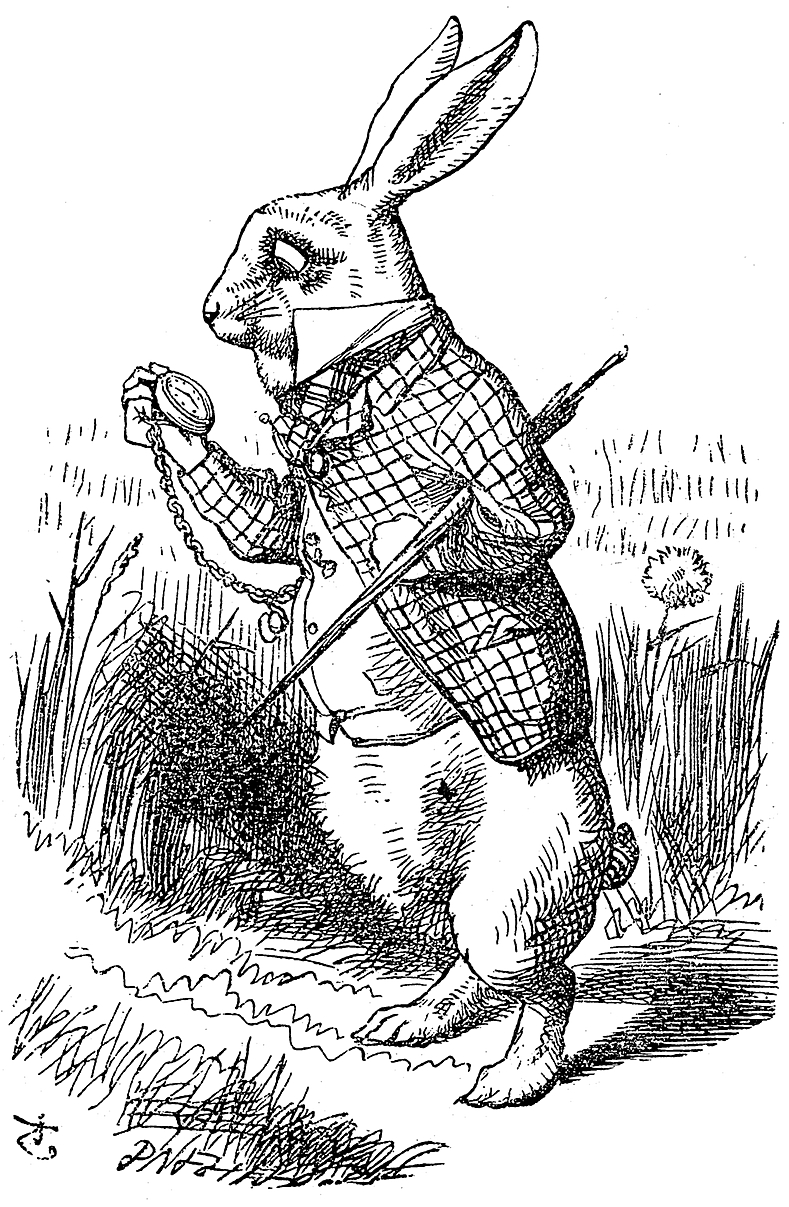
\includegraphics[height=5cm]{drawings/Alice-wr.jpg}

\textit{Oh dear! Oh dear! I shall be too late!}\\
\begin{small}
The White Rabbit in charge of real time
\end{small}
\end{center}
\end{frame}


\begin{frame}{Development model}
\begin{itemize}
\item Developed in the frame of ACCOR project
\item Open source design done in collaboration with industry
\item Commercial production and support
\end{itemize}
\end{frame}

\begin{frame}{Why White Rabbit?}
\begin{block}{General Machine Timing limitations}
\begin{itemize}
\item Low speed (500 kbps)
\item Lack of bidirectional communication
\item Complicated maintenance
\end{itemize}
\end{block}
\end{frame}

\begin{frame}{What is White Rabbit?}
\begin{center}
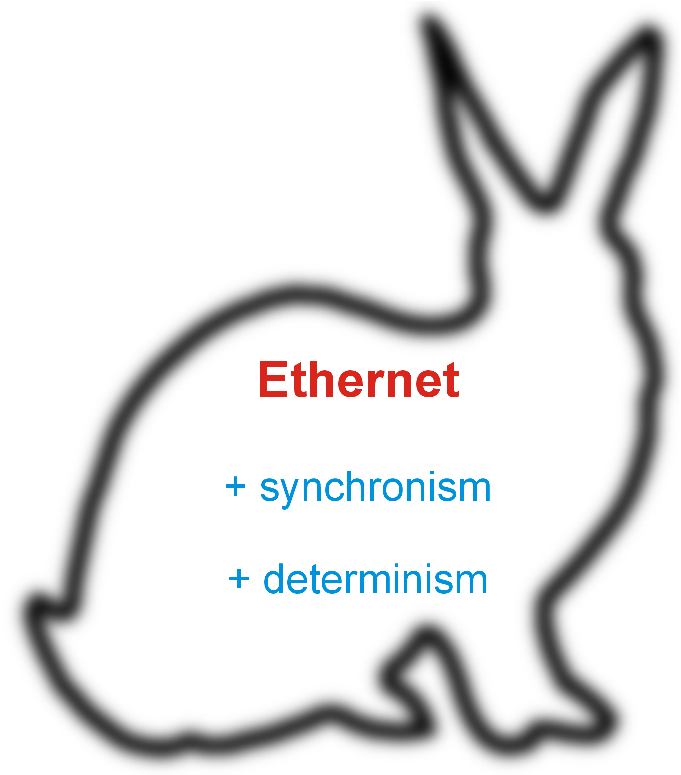
\includegraphics[height=6.5cm]{drawings/rabbit.png}
\end{center}
\end{frame}

\frame
{
  \frametitle{What is White Rabbit?}

% Extracting the clock from Ethernet carrier
\begin{block}{}
  An \textbf{extension} to \textbf{Ethernet} which provides:
  \begin{itemize}
% sync mode: - async & sync comparison, tree structure, common clock coming from single source, CDR
% advantage - easy  and precise implementation of time sync
  \item \textbf{Synchronous mode} (Sync-E) - common clock for physical layer in entire network, allowing for precise time and frequency transfer.

\item \textbf{Deterministic routing} latency - a guarantee that packet transmission delay between two stations will never exceed a certain boundary.
\end{itemize}
\end{block}

}

\begin{frame}{Design goals}
\begin{block}{Scalability}
Up to 2000 nodes.
\end{block}

\begin{block}{Range}
10 km fiber links.
\end{block}

\begin{block}{Precision}
1 ns time synchronization accuracy, 20 ps jitter.
\end{block}

\end{frame}

\section{Technology overview}

\frame{
  \frametitle{Technologies used in White Rabbit}
  Sub-nanosecond synchonization in WR is achieved by using the following three technologies together:
  \begin{itemize}
  \item Precision Time Protocol (IEEE1588)
  \item Synchronous Ethernet
  \item DMTD phase tracking
\end{itemize}
}

\frame{
\frametitle {Network topology}
% data traffic - no hierarchy, timing traffic - hierarchy	
\begin{center}
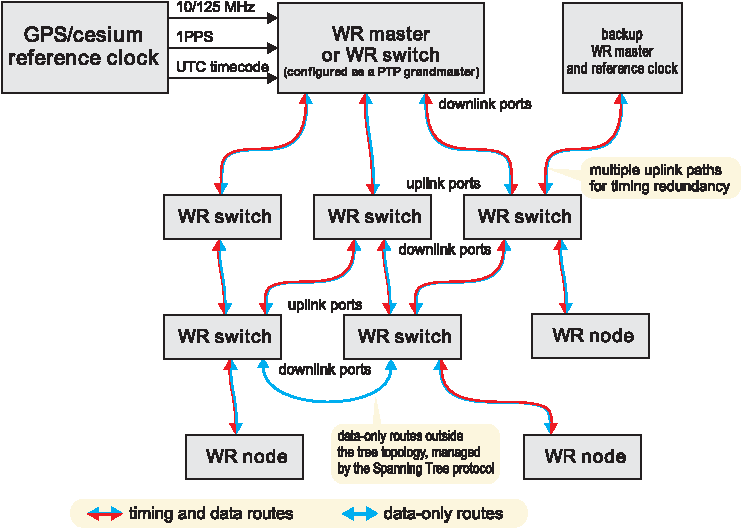
\includegraphics[height=6cm]{drawings/hierarchy.pdf}
\end{center}
}

\subsection{Precision Time Protocol (IEEE1588)}
\frame{
\frametitle{PTP Protocol (IEEE1588)}
\begin{block}{PTP}
Synchronizes local clock with the master clock by measuring and compensating the delay introduced by the link.
\end{block}

\begin{block}{Packet timestamping}
Link delay is measured by exchanging packets with precise hardware transmit/receipt timestamps
\end{block}
}

\frame{
\frametitle{PTP Protocol (IEEE1588)}
\begin{columns}[c]
\column{1.5in}
\begin{center}
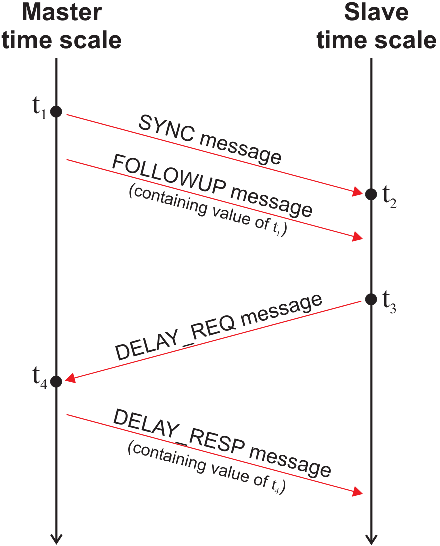
\includegraphics[height=5cm]{drawings/ptp_exchange.pdf}
\end{center}
\column{2.5in}
Having values of $t_{1}...t_{4}$, slave can:
\begin{itemize}
\item calculate one-way link delay: $\delta_{ms} = \frac{(t_{4}-t_{1}) - (t_{3}-t_{2})}{2}$
\item syntonize its clock rate with the master by tracking the value of $t_{2} - t_{1}$
\item compute clock offset: $offset = t_{2} - t_{1} + \delta_{ms}$
\end{itemize}
\end{columns}
}

\frame{
\frametitle{Disadvantages of traditional PTP}
  \begin{itemize}
    \item 
      All nodes have free-running oscillators
    \item
      Frequency drift has to be continously compensated, causing lots of network traffic
    \item
      That doesn't go well with determinism...
  \end{itemize}
}

% Extracting clock from the data - timing idea applied to network.
% gigabit PHYs - easy to get good quality clock
\subsection{Synchronous Ethernet}
\frame{
  \frametitle {Synchronous Ethernet}
	
  \begin{block}{Common clock for the entire network}
    \begin{itemize}
	 \item All network nodes use the same physical layer clock, generated by the System Timing Master
         \item Clock is encoded in the Ethernet carrier and recovered by the receiver chip (PHY).
         \item PTP is used only for compensating clock offset.
         \item Having the same clock frequency everywhere enables phase detector technology as the means of measuring time.
         \end{itemize}
       \end{block}
}

\frame{
\frametitle {Synchronous Ethernet}
\begin{center}
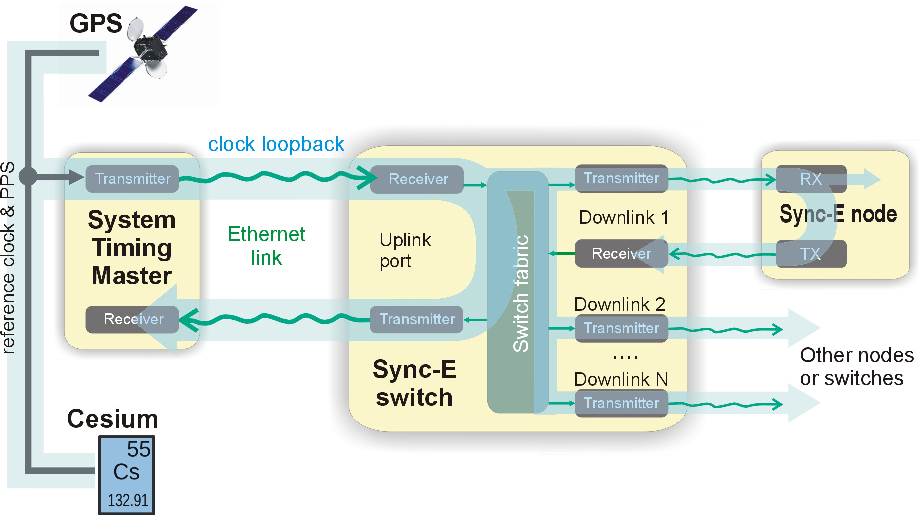
\includegraphics[height=6cm]{drawings/synce.png}
\end{center}
}

\subsection{Phase tracking}
\frame{
\frametitle{Phase tracking}
\begin{block}{Plain PTP}
PTP alone is not enough if we want very good accuracy, because of the granularity of the timestamps.
\end{block}


\begin{block}{Solution}
Measure the phase shift between transmit and receive clock on the master side, taking the advantage of Synchronous Ethernet.
\end{block}
}

\frame{
\frametitle {Phase tracking}

\begin{center}
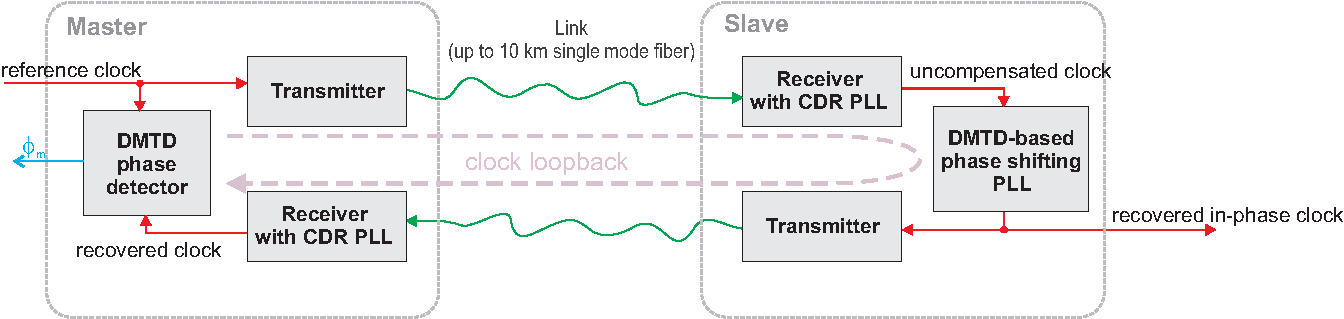
\includegraphics[height=2.5cm]{drawings/phase_tracking.pdf}
\end{center}

\begin{itemize}
\item
  Monitor phase of bounced-back clock continuously
\item
  Phase-locked loop in the slave follows the phase changes measured by the master
\end{itemize}
}

%\begin{frame}{Digital Dual Mixer Time Domain (DMTD) phase detector}
%\begin{center}
%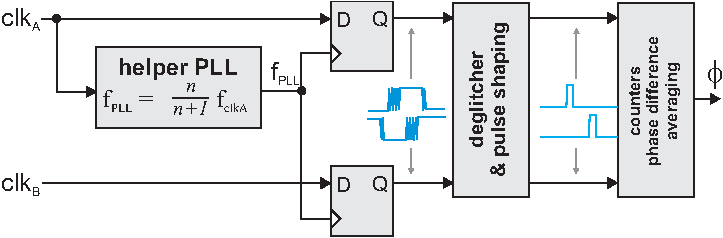
\includegraphics[width=\columnwidth]{dmtd.pdf}
%\end{center}
%\begin{itemize}
%\item Fully digital, so fully linear
%\item In a loop, it becomes a linear phase shifter
%\item Can handle multiple channels without need for extra hardware
%\end{itemize}
%\end{frame}

%\begin{frame}{Dealing with link asymmetry}
%  \begin{columns}[c]
%    \column{2in}
%    \begin{center}
%      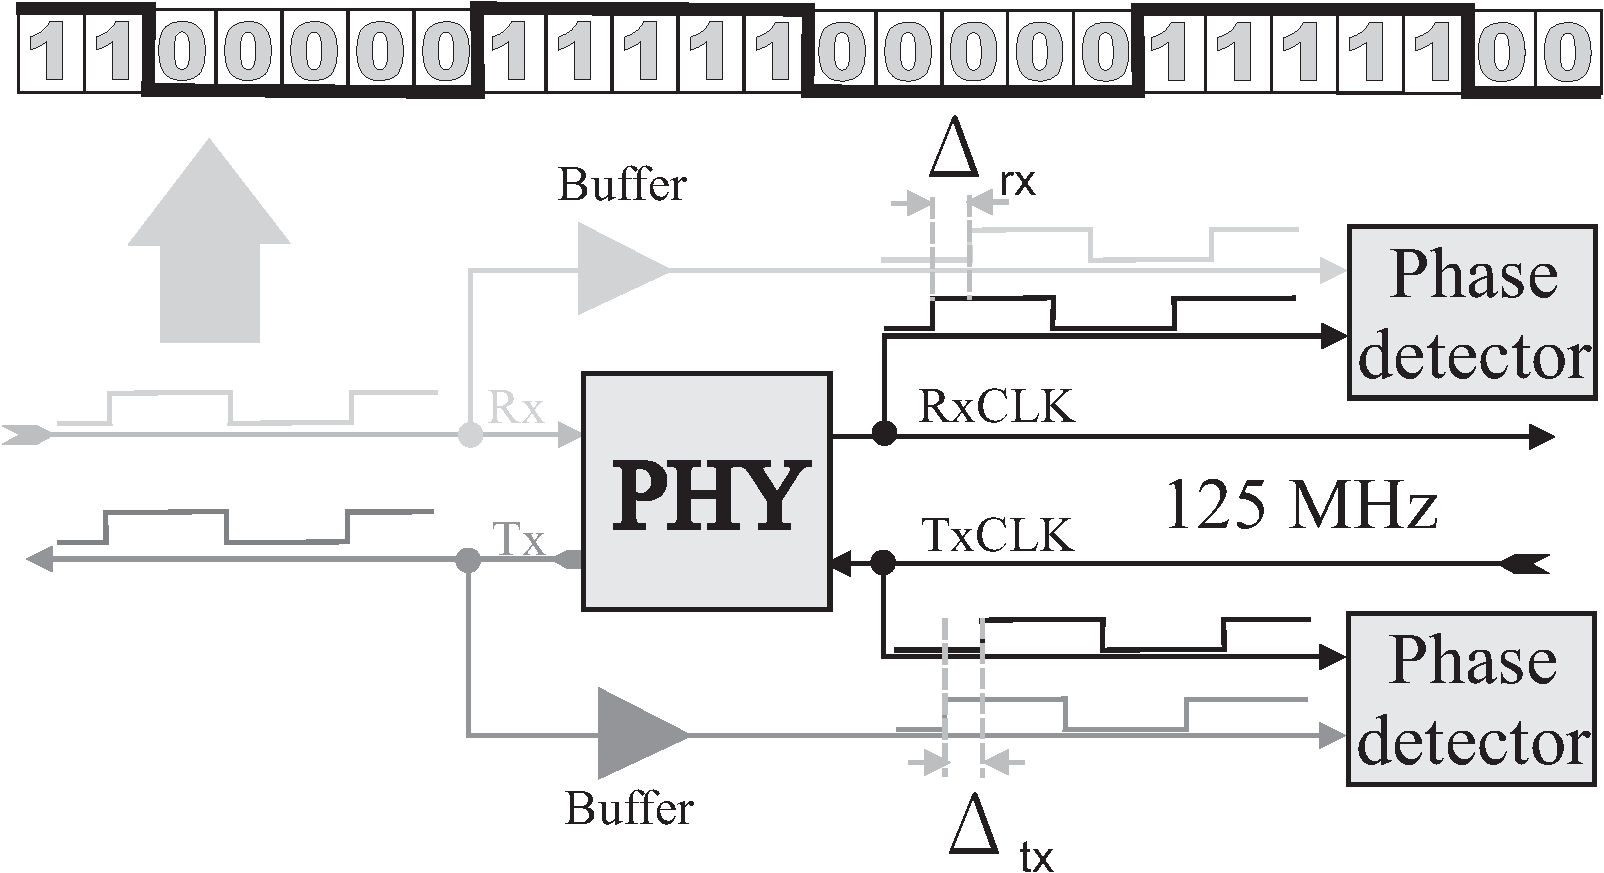
\includegraphics[height=3cm]{calibration.png}
%    \end{center}
%    PHY TX/RX latencies differ between each power-up cycle, but they can be measured using a DMT%D and a crosspoint switch.
%    \column{2in}

%    \begin{center}
%      \includegraphics[height=1.7cm]{model.png}
%    \end{center}
%    Fiber delay asymmetry is caused by difference in wavelengths for upstream and downstream tra%ffic and it increases linearly with link length.
%  \end{columns}
%\end{frame}

\subsection {White Rabbit Switch}


\begin{frame}{White Rabbit Switch}
\begin{center}
\includegraphics[width=8.5cm]{drawings/switch.jpg}
\end{center}
\begin{itemize}
\item Central element of WR network
\item Fully custom design, designed from scratch
\item 10 1000Base-LX ports, capable of driving 10 km of SM fiber
\item 200 ps synchronization accuracy
\end{itemize}
\end{frame}

\begin{frame}{White Rabbit Switch}
\begin{itemize}
\item Designed in microTCA MCH (Management Carrier Hub) format.
\item Multi-PCB design: base board with main big FPGA and CPU and Clocking Mezzanine, which handles the timing.
\item Can work in standalone mode (without a microTCA crate) via mini-backplane.
\end{itemize}
\end{frame}

\begin{frame}{Switch block diagram - main part}
\begin{center}
\includegraphics[width=9.5cm]{drawings/fpga_diagram.pdf}
\end{center}
\begin{itemize}
\item System FPGA handles all packet processing
\item CPU implements PTP stack and management functions (SNMP, Spanning Tree)
\end{itemize}
\end{frame}

\section{Applications}

\begin{frame}{Possible applications of White Rabbit}
\begin{center}
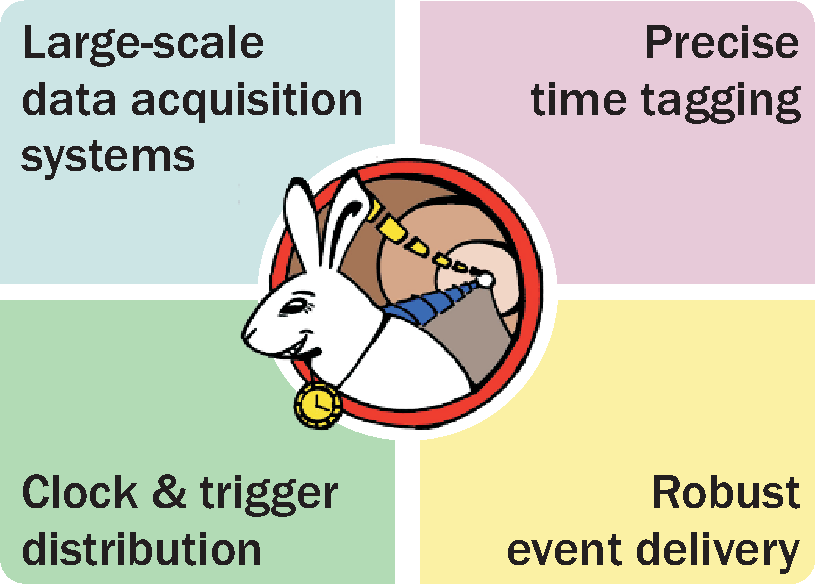
\includegraphics[width=7.5cm]{drawings/wr_apps.pdf}
\end{center}
\end{frame}


\subsection{WR in Co-HT's Hardware Kit}
\begin{frame}{WR in Co-HT's Hardware Kit}
\begin{center}

  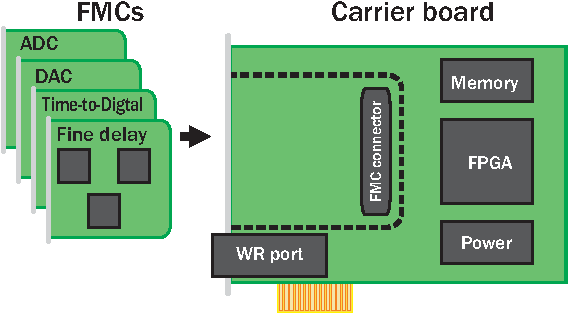
\includegraphics[width=6cm]{drawings/shw_kit}

  \begin{block}{Co-HT FMC-based Hardware Kit:}
    \begin{itemize}
    \item FMCs (FPGA Mezzanine Cards) with ADCs, DACs, TDCs, fine delays, digital I/O
    \item Carrier boards in PCI-Express, VME and uTCA formats
    \item All carriers are equipped with a White Rabbit port
    \end{itemize}
  \end{block}

\end{center}
\end{frame}


\begin{frame}{Ethernet Clock distribution a.k.a. Distributed DDS}
  \begin{center}
    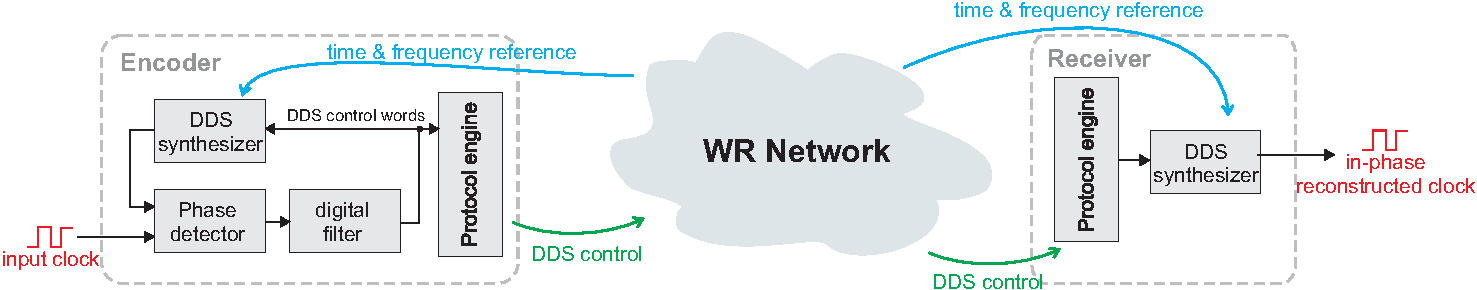
\includegraphics[width=\columnwidth]{drawings/remote_dds.pdf}
  \end{center}
  \begin{block}{Distributed Direct Digital Synthesis}
    \begin{itemize}
    \item Replaces dozens of cables with a single fiber
    \item Works over big distances without degrading signal quality
    \item Can provide various clocks (TTC, RF, bunch clock) with a single, standarized link
    \end{itemize}
  \end{block}
\end{frame}


\begin{frame}{Distributed oscilloscope}
  \begin{center}
    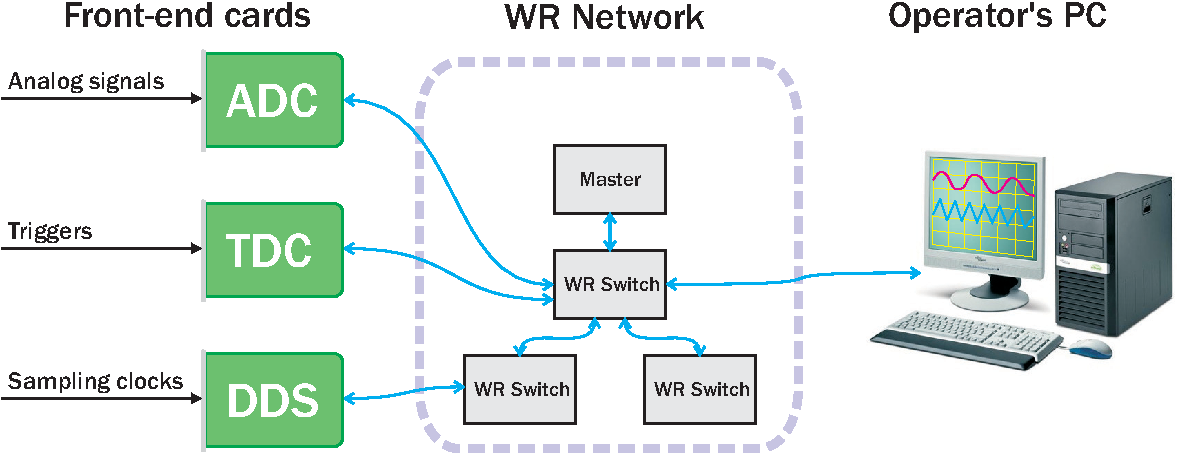
\includegraphics[width=8cm]{drawings/distr_oscill}
    \end{center}
    \begin{block}{}
      \begin{itemize}
      \item Common clock in the entire network: no skew between ADCs
      \item Ability to sample with different clocks via Distributed DDS
      \item External triggers can be time tagged with a TDC and used to reconstruct the original time base in the Operator's PC.
      \end{itemize}
    \end{block}
\end{frame}



\section{Planning}

\subsection{Current status}

\begin{frame}{WR Switch development status}
	\begin{block}{Switch hardware}
          \begin{itemize}
            \item Working and debugged V2 hardware prototype
            \item Tested on 10-km fiber links
            \item Interoperates with standard Ethernet gear
            \end{itemize}
            \end{block}

	\begin{block}{Switch software}
          \begin{itemize}
            \item Done the Hardware Abstraction Layer and PTP daemon 
            \item Sub-nanosecond accuracy over PTP has been achieved
            \item Verified interoperability with other PTP devices on ISPCS 2010 Plug Fest
            \end{itemize}
          \end{block}
\end{frame}

\begin{frame}{Already achieved...}
  \begin{block}{According to ISPCS Plug Fest results ...}
    \begin{center}
      \textbf{... White Rabbit is the most accurate PTP implementation in the world!}
  \end{center}
  \end{block}
\end{frame}

\subsection{Development plans for Q4 2010 and 2011}

\begin{frame}{CERN - White Rabbit developers}
  \begin{block}{T. Wlostowski}
    \begin{itemize} 
      \item HDL development 
      \item Further improvements in the synchronization performance
      \item Co-design of V3 Switch hardware with the industrial partners
      \end{itemize}
    \end{block}
  \begin{block}{M. Lipinski}
    \begin{itemize} 
      \item Development of fault-proof event delivery protocol
      \item PTP stack support
      \item HDL development
      \end{itemize}
    \end{block}
\end{frame}

\begin{frame}{External contributors}

  \begin{block}{GSI Darmstadt}
    \begin{itemize} 
    \item Fieldbus protocol development, working on reliability
    \item HDL development
      \end{itemize}
    \end{block}
  \begin{block}{Alessandro Rubini (GNUDD)}
    \begin{itemize} 
      \item Main software developer
      \item Device drivers
      \item Embedded Linux support
      \end{itemize}
    \end{block}
\end{frame}

\begin{frame}

  \begin{block}{Integrasys}
    \begin{itemize} 
      \item Development of switch management software
      \item IEEE802.x compatibility testing
      \end{itemize}
    \end{block}

  \begin{block}{Seven Solutions}
    \begin{itemize} 
      \item Co-design of V3 switch hardware (technical spec available mid-November)
      \item Prototype production and testing
      \end{itemize}
    \end{block}

  \begin{block}{Elproma (not confirmed yet)}
    \begin{itemize} 
      \item Commercial WR OEM modules and time servers
      \end{itemize}
    \end{block}

\end{frame}

\begin{frame}{Foreseen milestones}

  \begin{block}{WR Switch}
    \begin{itemize} 
      \item Full basic functionality of HDL and software: mid-December 2010
      \item V3 prototype: Q3 2011
      \item Commercial product: Q1 2012
      \end{itemize}
    \end{block}

  \begin{block}{WR Ecosystem}
    \begin{itemize} 
      \item FMC Carriers: VME version prototype done, PCIe available at the end of November
      \item WR timing node: Q2 2012
      \item Mezzanines: Full set of cards available Q4 2011 
      \end{itemize}
    \end{block}

\end{frame}


\begin{frame}{Summary}
  % Keep the summary *very short*.
  \begin{itemize}
  \item
    A data link fulfilling all our needs in \textbf{synchronization} and \textbf{determinism}.
  \item
    A successful \textbf{collaboration} including institutes and companies.
  \item
    Full system available at the \textbf{middle of 2012}
  \end{itemize}
\end{frame}

\end{document}
